\documentclass{article}
\usepackage[utf8]{inputenc}

\title{Background Study on MeerKAT SETI Search}
\author{Jiapeng Zhang}
\date{May 2021}

\usepackage{natbib}
\usepackage{graphicx}
\usepackage{float}

\begin{document}

\maketitle

\section{Introduction}
In the universe, numerous signals are in the form of electromagnetic(EM) waves, such as communication signals, These signals are strongly coherent, which means the power spectrum of such signals would be a narrow band. However, these signals will show a drift rate with respect to time, when detecting, due to Doppler effect. Therefore, Search for Extraterrestrial Intelligence(SETI) is a research based on analyzing the drift rate to seek possible transmitter signals from exoplanets. Currently, The research is being conducted on MeerKAT. It is a large radio telescope array focusing, which mainly detects two bands of signals - one is 856-1712MHz and another is 544-1088MHz. In this report, it is primarily centered on the basic understanding of SETI.

\section{Theory}
In order to conclude all the possible signals, maximum drift rate is the foremost variables studied. To calculate the maximum drift rate, there are four dominant factors:
    1.Rotational acceleration of Earth
    2.Orbital acceleration of Earth
    3.Rotational acceleration of the observed object
    4.Orbital acceleration of the observed object
Based on the above, the maximum drift rate is given by,
\begin{equation}
    \centering
    \dot{f}=\frac{f_{rest}}{c}(\frac{4\pi^2R_{\oplus}}{P_{rot,\oplus}^2}+\frac{4\pi^2R}{P_{rot}^2}+\frac{GM_\odot}{r_\oplus^2}+\frac{GM}{r^2})
\end{equation}
where $f_{rest}$ is the minimal detectable frequency, $r$ and $r_\oplus$ are the orbital radius of the observed object and Earth, $R$ and $R_\oplus$ are the radii of the observed object and Earth, $P_{rot}$ and $P_{rot,\oplus}$ are the rotation period of the observed object and Earth.\cite{2019ApJ...884...14S}

\section{Known Objects}
By applying equation 1 to a few know objects,

\begin{table}
\centering
\resizebox{\textwidth}{!}{
\begin{tabular}{l|rrrrrr}
\hline
         Name &  r\_obs(km) &  P\_obs(day) &     R\_obs(km) &  M\_center(Kg) &  drift\_rate\_1 &  drift\_rate\_2 \\
\hline
        Earth &     6371.0 &       1.000 &  1.496e+08 &  1.989e+30 &      0.226125 &      0.143706 \\
         Moon &     1737.1 &      27.322 &  3.844e+05 &  5.972e+24 &      0.120794 &      0.076767 \\
      Mercury &     4880.0 &      58.646 &  5.791e+07 &  1.989e+30 &      0.226034 &      0.143648 \\
      Jupiter &    69911.0 &       0.414 &  7.786e+11 &  1.989e+30 &      6.268084 &      3.983455 \\
           Io &     1821.6 &       1.769 &  4.217e+05 &  1.898e+27 &      2.154424 &      1.369167 \\
  51 Pegasi b &   135830.0 &      21.900 &  7.880e+06 &  2.208e+30 &      6.889148 &      4.378150 \\
 Tau Boötis b &    11945.6 &       3.310 &  9.343e+11 &  2.765e+30 &      0.129515 &      0.082309 \\
   Beta Pic b &   102070.1 &       0.338 &  1.376e+09 &  3.481e+30 &     13.595275 &      8.639988 \\\hline
\end{tabular}}
\caption{A few known objects and their drift rate under two different bands.}
\label{table:1}
\end{table}

\begin{figure}[H]
\centering
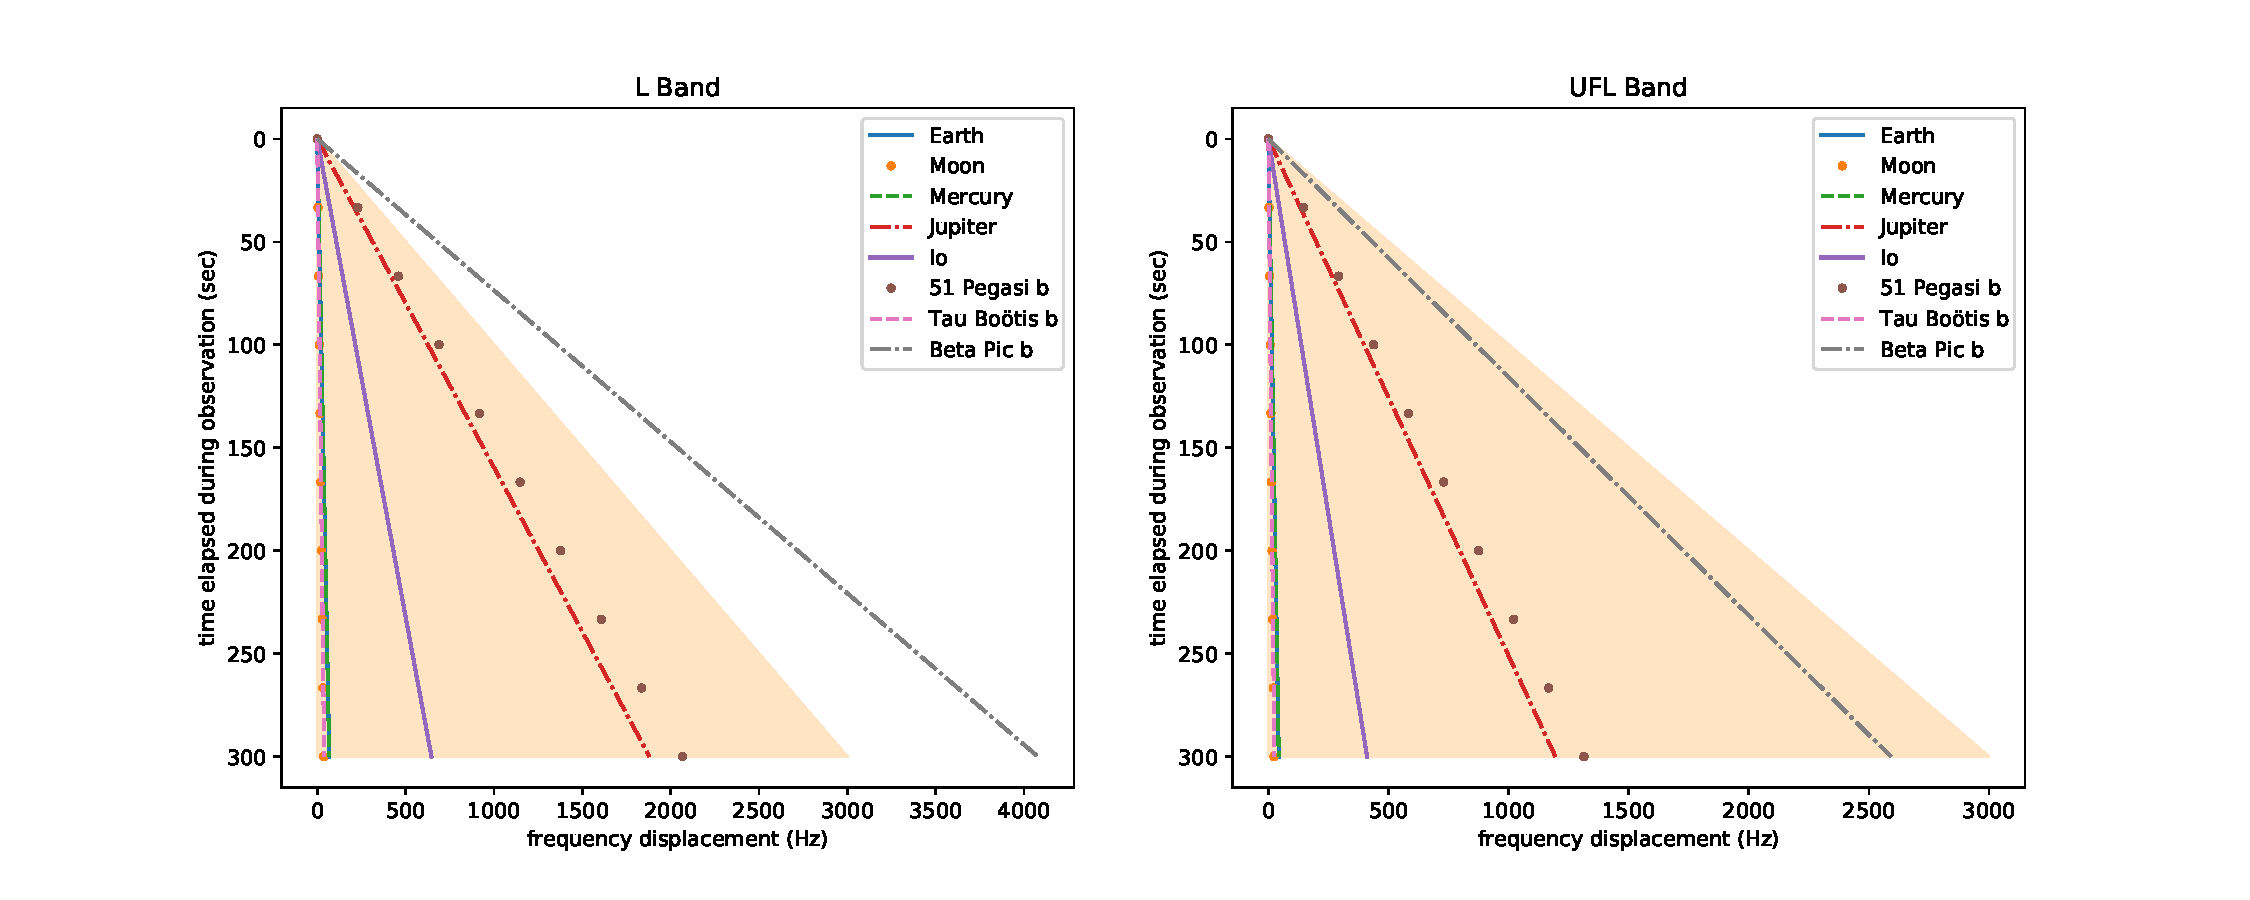
\includegraphics[scale=0.3]{Part_1.pdf}
\caption{A simulation of 5 mins observation of narrow bandwidths for various drift rate, starting at $f_{rest}=856MHz$(left) and $f_{rest}=544MHz$(right). The shaded area is where the drift rate is 10Hz/s.}
\label{fig:1}
\end{figure}

From fig.1, it is clearly that 10Hz/s of drift rate is not enough, even for known objects. The maximum drift rate during 5 mins for L band is 2.853 MHz/s, and for UFL band is 1.813 MHz/s.

\section{Voyager}
Voyager has collected a significantly large amount of signals. Here are two plots of time and power with respect to a range of frequency from 8418.457034043968 MHz to 8421.38671875 MHz

\begin{figure}[H]
    \centering
    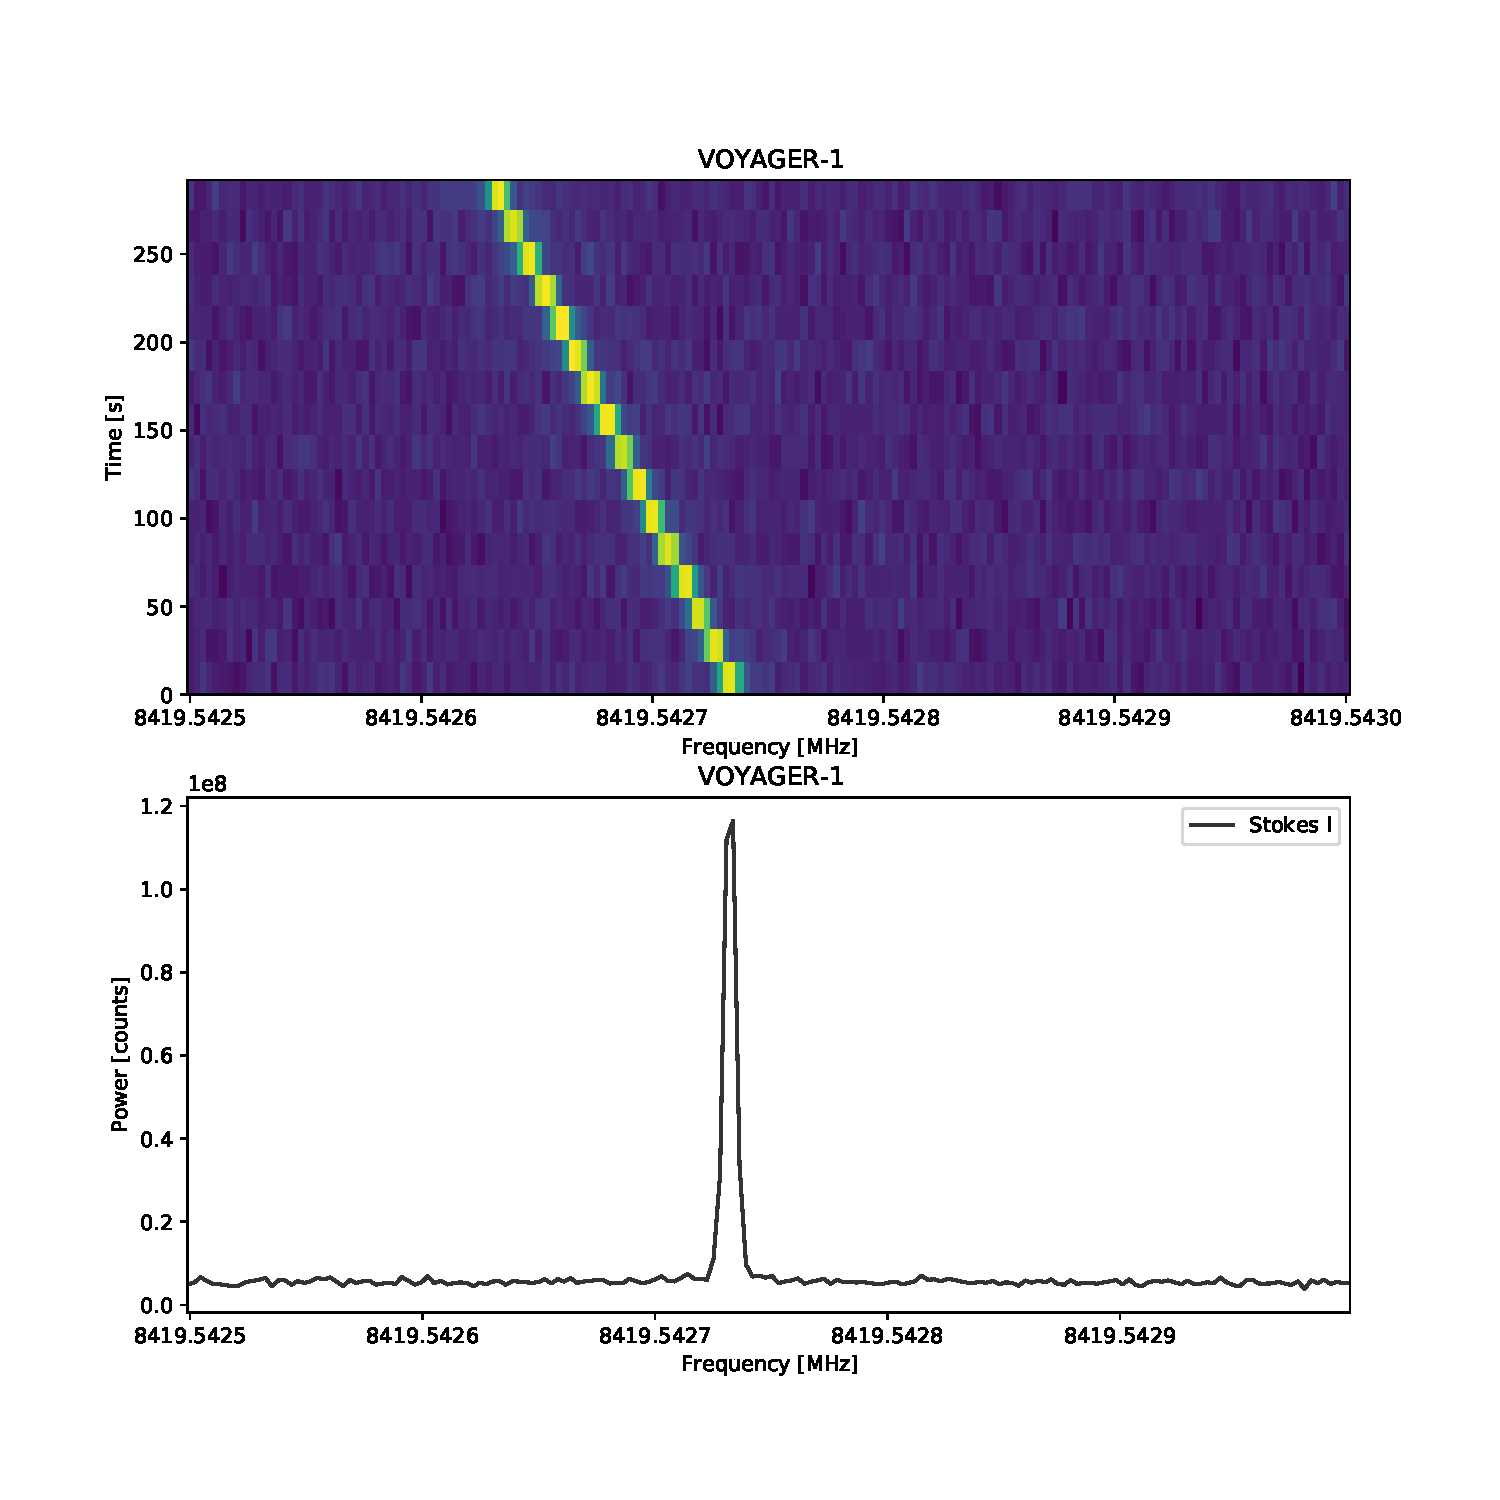
\includegraphics[scale=0.4]{voyager.pdf}
    \caption{The collected data from voyager from 8418.457034043968 MHz to 8421.38671875 MHz. The figure above is the time elapsed vs frequency, and the figure below is the power vs frequency.}
    \label{fig:2}
\end{figure}

In Sheikh et al., it was suggested that above 200nHz of normalized drift rate is worth further study. From this range of frequency. The drift rate 0.363527 Hz/s. If MeerKAT is used, the normalized drift rate is 0.425 nHz for L band and 0.668 nHz. MeerKAT won't detect such signal because it exceeds the bandwidth. It is not compatible with what Sheikh et al. range.

\section{Extension}
Due to the lack of access to off-satellite MeerKAT observation data, there is only the power spectrum plot of the on-satellite data.

\begin{figure}[H]
    \centering
    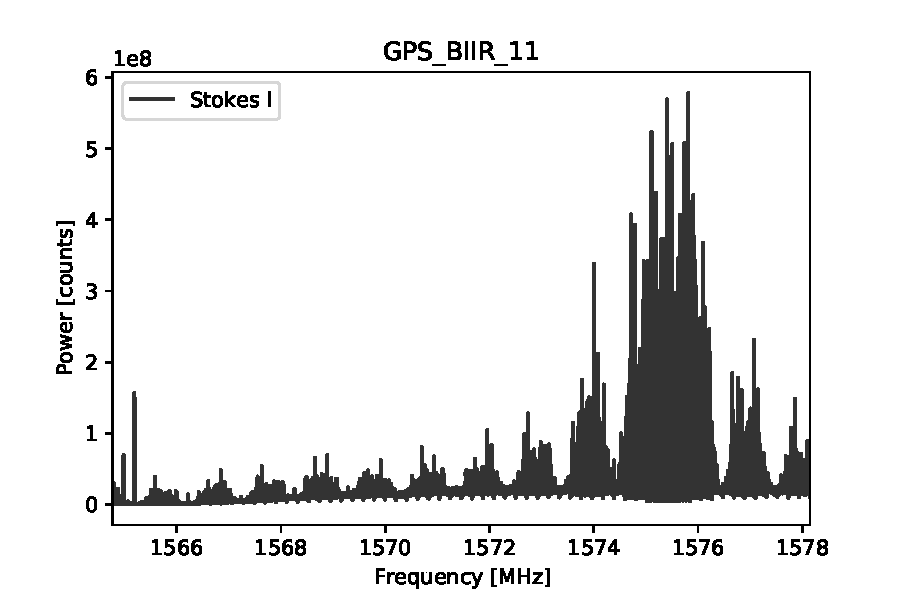
\includegraphics[scale=0.8]{on.pdf}
    \caption{On-satellite signal power spectrum from MeerKAT.}
    \label{fig:3}
\end{figure}

\begin{figure}[H]
    \centering
    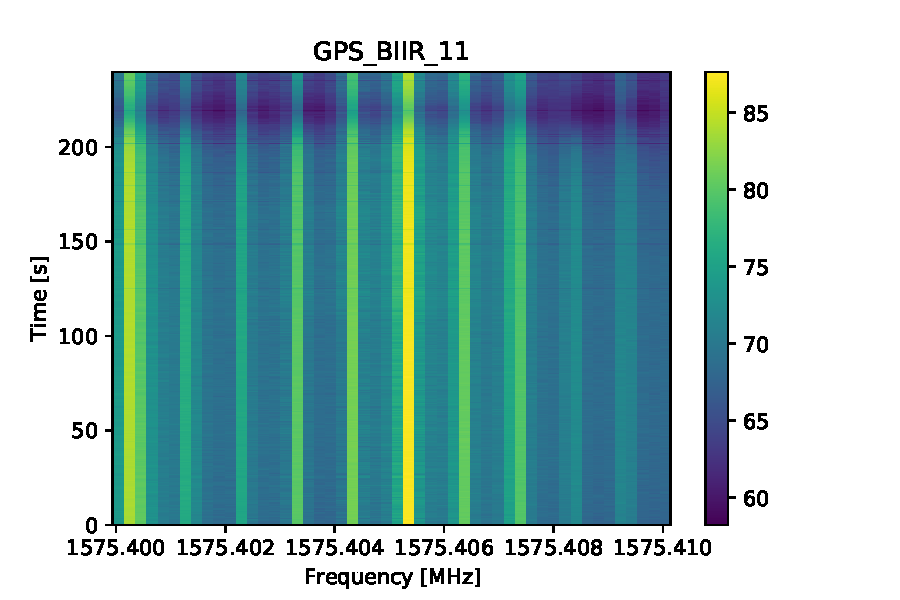
\includegraphics[scale=0.8]{on_waterfall.pdf}
    \caption{On-satellite signal waterfall from MeerKAT.}
    \label{fig:4}
\end{figure}

The drift rate for this satellite signal is significantly small to be recognized. The frequency at 1575.4055MHz is most likely to be compromised by Radio Frequency Interference

\bibliographystyle{plain}
\bibliography{export-bibtex.bib}

\end{document}
